\section{Results}\label{sec:results}

\subsection{Model Comparison}

Table~\ref{tab:model_comparison} summarises test-set performance for all eight configurations, sorted by RMSE. CatBoost-PPSO clearly separates itself from the rest, while the remaining models cluster relatively tightly---with Linear Regression, notably, sitting among the tree-based methods rather than trailing behind them.

\begin{table}[H]
\centering
\caption{Model comparison on the test set (213 samples).}
\label{tab:model_comparison}
\begin{tabular}{@{}lrrrrrr@{}}
\toprule
\textbf{Model} & \textbf{MAE} & \textbf{RMSE} & \textbf{$R^2$} & \textbf{MAPE (\%)} & \textbf{RAE} & \textbf{WI} \\
\midrule
CatBoost-PPSO & \textbf{1{,}496.2} & \textbf{1{,}895.5} & \textbf{0.9135} & \textbf{0.89} & \textbf{0.280} & \textbf{0.9774} \\
CatBoost & 1{,}679.4 & 2{,}118.8 & 0.8919 & 0.99 & 0.314 & 0.9709 \\
Linear Reg. & 1{,}693.4 & 2{,}119.2 & 0.8919 & 1.01 & 0.317 & 0.9731 \\
XGB-PPSO & 1{,}687.8 & 2{,}165.6 & 0.8871 & 1.00 & 0.315 & 0.9697 \\
Random Forest & 1{,}774.0 & 2{,}237.6 & 0.8795 & 1.05 & 0.332 & 0.9653 \\
RF-PPSO & 1{,}794.1 & 2{,}283.9 & 0.8744 & 1.06 & 0.335 & 0.9634 \\
XGBoost & 1{,}833.4 & 2{,}313.4 & 0.8712 & 1.08 & 0.343 & 0.9652 \\
\bottomrule
\end{tabular}
\end{table}

Key observations:

\begin{enumerate}
    \item \textbf{CatBoost-PPSO leads on every metric}: $R^2 = 0.914$ (over 91\% of demand variance explained), RMSE of 1{,}895.5\,MWh ($\approx$1.1\% of mean daily demand), and MAPE of 0.89\%.
    \item \textbf{PPSO gains are model-dependent.} Tuning improves CatBoost substantially (RMSE $-$10.5\%) and XGBoost moderately ($-$6.4\%), but slightly hurts Random Forest ($+$2.1\%)---likely because RF's bagging mechanism is already robust to hyperparameters, and the optimiser overfits the cross-validation folds. Since every model received the same budget, these differences confirm that CatBoost-PPSO's lead is genuine, not a by-product of preferential tuning.
    \item \textbf{Linear Regression is surprisingly competitive}, essentially tied with default CatBoost on RMSE. This tells us that the engineered autoregressive features (lag-1, rolling means) already linearise much of the problem; the value of tree models lies in capturing residual weather--calendar interactions.
    \item \textbf{All models exceed $R^2 = 0.87$ and WI $= 0.96$}, which confirms that the 16-feature set captures the dominant demand drivers regardless of model choice.
\end{enumerate}

\subsection{Prediction Behaviour}

Figure~\ref{fig:predictions} plots actual versus predicted demand for CatBoost-PPSO across the 213-day test period. The model tracks weekly cyclicity well (weekend dips are clearly reproduced), follows demand level shifts, and tends to err most on sharp holiday-related drops---events that are hard to anticipate from weather and calendar features alone.

\begin{figure}[H]
    \centering
    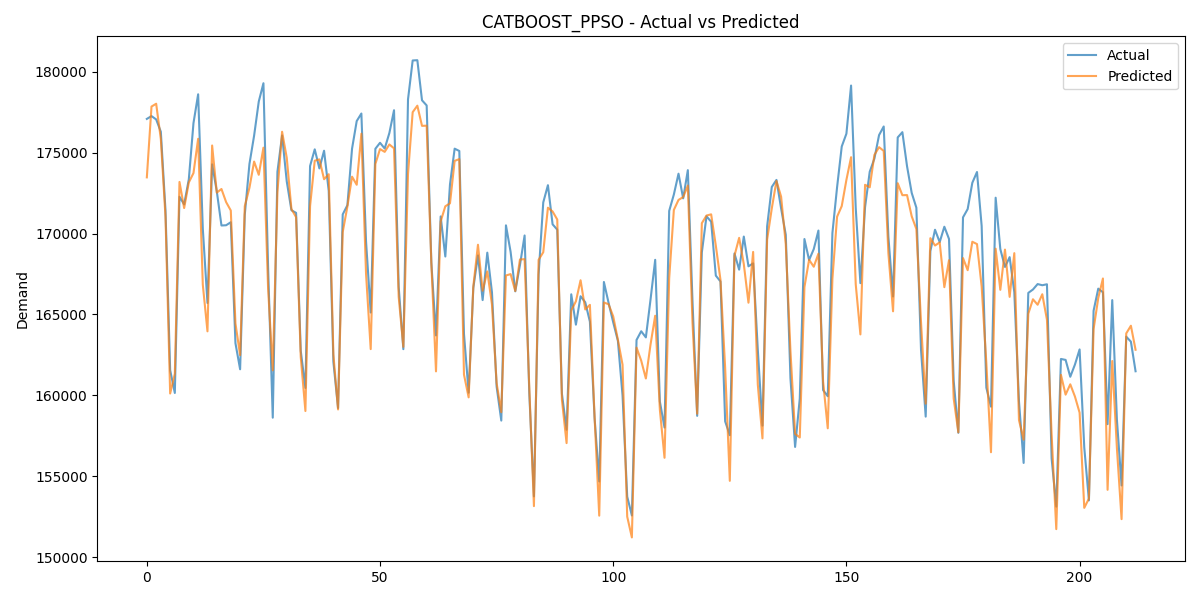
\includegraphics[width=0.88\textwidth]{eval/images/predictions_catboost_ppso.png}
    \caption{Actual vs.\ predicted daily electricity demand (MWh), CatBoost-PPSO, test set.}
    \label{fig:predictions}
\end{figure}

\subsection{Feature Importance}

Figure~\ref{fig:feature_importance} shows the CatBoost-PPSO importance scores. As expected, autoregressive features dominate---\texttt{demand\_lag\_1} and the rolling means carry the most weight---followed by \texttt{day\_of\_week}. Weather variables (temperature, humidity, CCI) sit in the mid-ranks, providing meaningful exogenous signal on top of the demand history. The same ranking holds for RF and XGBoost, suggesting this hierarchy is robust across model families.

\begin{figure}[H]
    \centering
    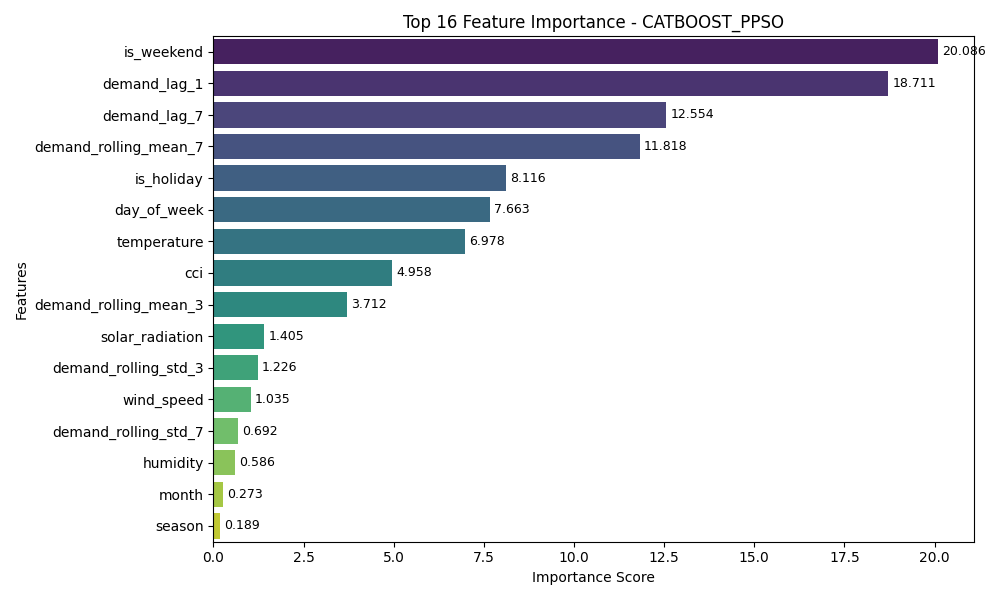
\includegraphics[width=0.78\textwidth]{eval/images/feature_importance_catboost_ppso.png}
    \caption{Feature importance, CatBoost-PPSO. Autoregressive features dominate, with weather variables providing secondary signal.}
    \label{fig:feature_importance}
\end{figure}

\subsection{Impact of PPSO Optimisation}

To isolate the tuning effect, Table~\ref{tab:ppso_impact} breaks down the before-and-after metrics for CatBoost, the model that benefited most.

\begin{table}[H]
\centering
\caption{Impact of PPSO hyperparameter optimisation on CatBoost.}
\label{tab:ppso_impact}
\begin{tabular}{@{}lrrr@{}}
\toprule
\textbf{Metric} & \textbf{CatBoost (default)} & \textbf{CatBoost-PPSO} & \textbf{Improvement} \\
\midrule
MAE (MWh) & 1{,}679.4 & 1{,}496.2 & $-$10.9\% \\
RMSE (MWh) & 2{,}118.8 & 1{,}895.5 & $-$10.5\% \\
$R^2$ & 0.8919 & 0.9135 & $+$2.2 pp \\
MAPE (\%) & 0.99 & 0.89 & $-$10.6\% \\
RAE & 0.314 & 0.280 & $-$10.9\% \\
WI & 0.971 & 0.977 & $+$0.6 pp \\
\bottomrule
\end{tabular}
\end{table}

Compared with Zhang et al.\ \parencite{zhang2023catboostppso}, who reported $R^2 = 0.971$ on hourly single-customer data, our lower $R^2$ (0.914) is not surprising: daily national demand aggregates consumption across millions of heterogeneous users, which inevitably adds unexplained variance. Still, the fact that the methodology transfers across such different scales, resolutions, and climates is encouraging.
